\section{Resultados}

\subsection{Bases de datos de respuestas al impulso}
Para tener una medida de la variedad de reverberación presente en los conjuntos de respuestas al impulso reales, generadas y aumentadas, se utilizan los parámetros $TR_mid$ y $DRR$. 

\begin{figure}[H]
	\centering{}
	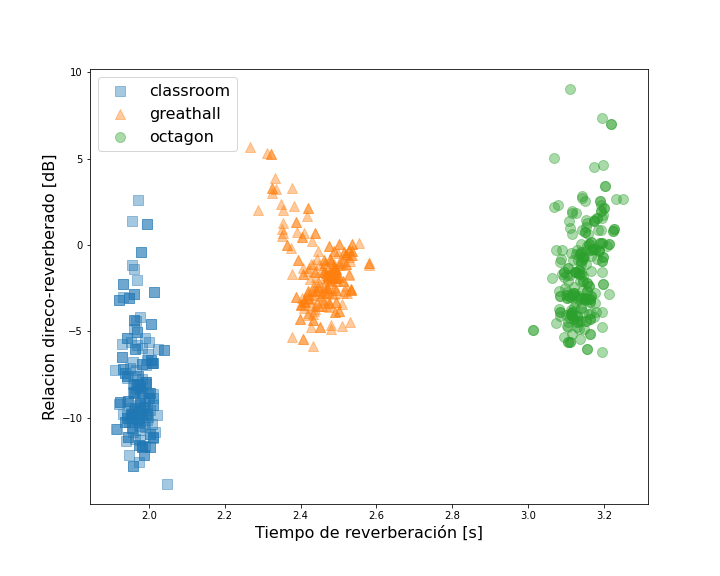
\includegraphics[scale=0.5]{reales.png}
	\caption{Conjunto de respuestas al impulso reales.}
	\label{fig:reales}
\end{figure}

\begin{figure}[H]
	\centering{}
	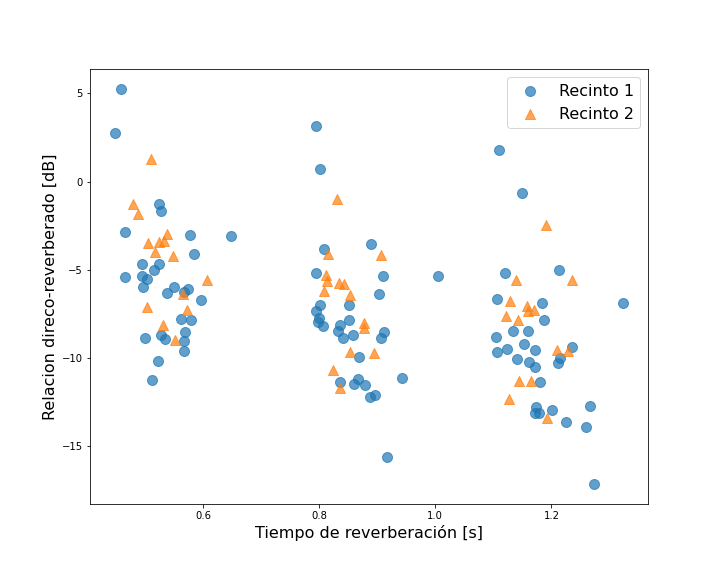
\includegraphics[scale=0.5]{generadas.png}
	\caption{Conjunto de respuestas al impulso generadas.}
	\label{fig:generadas}
\end{figure}

\begin{figure}[H]
	\centering{}
	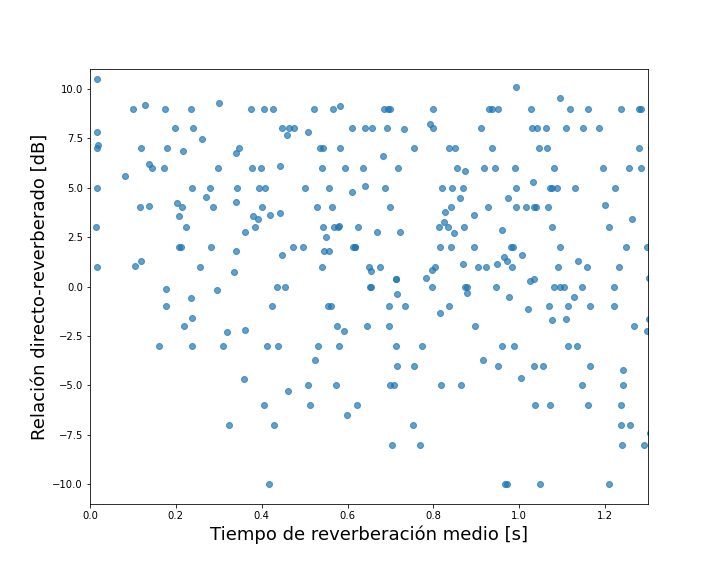
\includegraphics[scale=0.5]{aumentadas.png}
	\caption{Conjunto de respuestas al impulso aumentadas.}
	\label{fig:aumentas}
\end{figure}



\subsection{Conjuntos de datos reverberados}

Para las evaluaciones se tuvieron en cuenta tres conjuntos de datos de acuerdo al tipo de respuestas al impulso utilizadas para generar la reverberación: reales, generadas y aumentadas. Para medir el desempeño de la tarea de dereverberación, las metricas se evaluan sobre los conjuntos reverberados y luego sobre sus correspondientes resultados dereverberados. Los resultados de estas métricas para los conjuntos reverberados se puede observar en la tabla \ref{table:resultados_reverb}. 

\begin{table}[H]
\centering
\caption{Resultados de las metricas sobre los conjuntos reverberados}
\begin{tabular}{|c|c|c|c|}
\hline
Conjunto   & \textbf{SDR} & \textbf{SRMR} & \textbf{ESTOI} \\ \hline
Reales     & -7.35        & 1.61          & 0.27           \\
Generadas  & -4.12        & 3.08          & 0.40           \\
Aumentadas & -2.08        & 4.66          & 0.67           \\ \hline
\end{tabular}
\label{table:resultados_reverb}
\end{table}

\subsection{Funcionamiento del sistema}

\begin{figure}[H]
        \centering
        \begin{subfigure}[b]{0.475\textwidth}
            \centering
            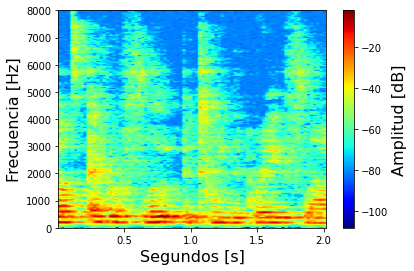
\includegraphics[width=\textwidth]{espectro_in.png}
            \caption[Network2]%
            {{\small Espectrograma reverberado}}    
            \label{fig:mean and std of net14}
        \end{subfigure}
        \hfill
        \begin{subfigure}[b]{0.475\textwidth}  
            \centering 
            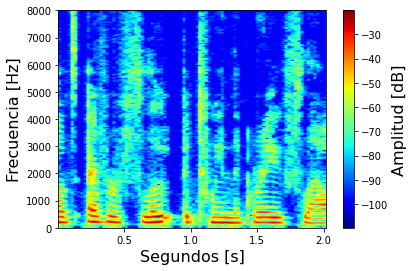
\includegraphics[width=\textwidth]{espectro_target.png}
            \caption[]%
            {{\small Espectrograma anecoico}}    
            \label{fig:mean and std of net24}
        \end{subfigure}
        \vskip\baselineskip
        \begin{subfigure}[b]{0.475\textwidth}   
            \centering 
            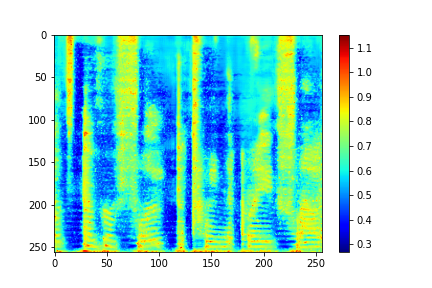
\includegraphics[width=\textwidth]{mascara.png}
            \caption[]%
            {{\small Mascara estimada por la red}}    
            \label{fig:mean and std of net34}
        \end{subfigure}
        \hfill
        \begin{subfigure}[b]{0.475\textwidth}   
            \centering 
            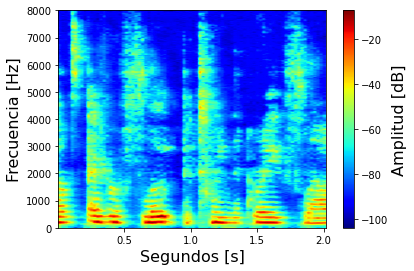
\includegraphics[width=\textwidth]{espectro_out.png}
            \caption[]%
            {{\small Espectrograma dereverberado}}    
            \label{fig:mean and std of net44}
        \end{subfigure}
        \caption[ The average and standard deviation of critical parameters ]
        {\small Ejemplo de procesamiento de audio reverberado} 
        \label{fig:mean and std of nets}
    \end{figure}

\subsection{Dereverberación del habla}

Los resultados obtenidos para el primer conjunto de pruebas definidos en la tabla \ref{tab:pruebas} se expresan en las figuras \ref{fig:1_SDR}, \ref{fig:1_SRMR} y \ref{fig:1_ESTOI} para las variaciones de las metricas SDR, SRMR y ESTOI respectivamente. 

\begin{figure}[H]
	\centering{}
	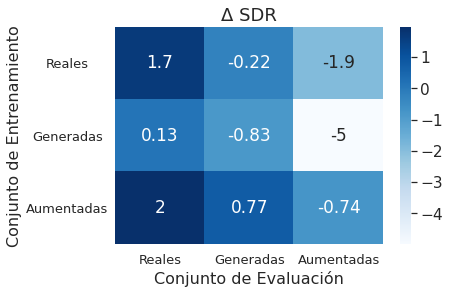
\includegraphics[scale=0.5]{prueba1_SDR.png}
	\caption{Variaciones de SDR para el primer conjunto de pruebas.}
	\label{fig:1_SDR}
\end{figure}

\begin{figure}[H]
	\centering{}
	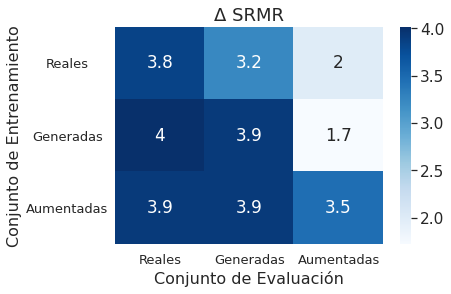
\includegraphics[scale=0.5]{prueba1_SRMR.png}
	\caption{Variaciones de SRMR para el primer conjunto de pruebas.}
	\label{fig:1_SRMR}
\end{figure}

\begin{figure}[H]
	\centering{}
	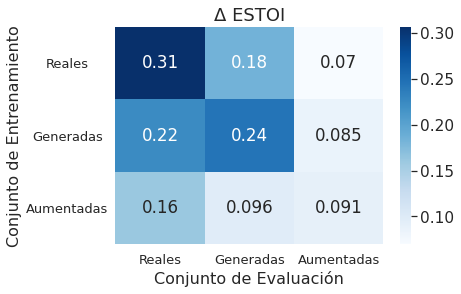
\includegraphics[scale=0.5]{prueba1_ESTOI.png}
	\caption{Variaciones de ESTOI para el primer conjunto de pruebas.}
	\label{fig:1_ESTOI}
\end{figure}

Los resultados correspondientes al segundo conjunto de pruebas definido en la tabla \ref{tab:pruebas_combinadas} se muestran en las figuras \ref{fig:2_SDR}, \ref{fig:2_SRMR} y \ref{fig:2_ESTOI} para las variaciones de las metricas SDR, SRMR y ESTOI respectivamente.

\begin{figure}[H]
	\centering{}
	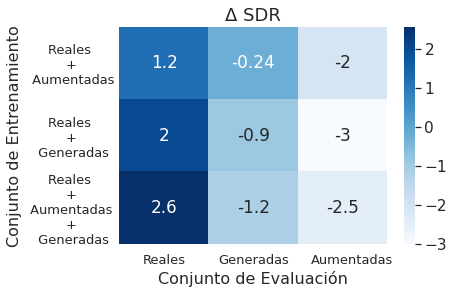
\includegraphics[scale=0.5]{prueba2_SDR.png}
	\caption{Variaciones de SDR para el segundo conjunto de pruebas.}
	\label{fig:2_SDR}
\end{figure}

\begin{figure}[H]
	\centering{}
	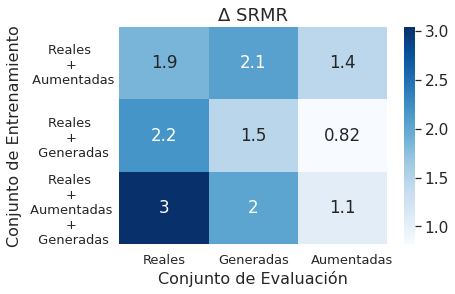
\includegraphics[scale=0.5]{prueba2_SRMR.png}
	\caption{Variaciones de SRMR para el segundo conjunto de pruebas.}
	\label{fig:2_SRMR}
\end{figure}

\begin{figure}[H]
	\centering{}
	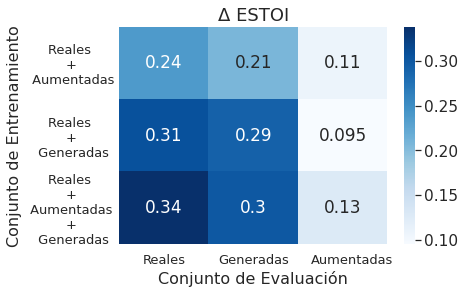
\includegraphics[scale=0.5]{prueba2_ESTOI.png}
	\caption{Variaciones de ESTOI para el segundo conjunto de pruebas.}
	\label{fig:2_ESTOI}
\end{figure}

